\documentclass{../source/Experiment}

\major{信息工程}
\name{}
\title{基4-FFT算法编程}
\stuid{}
\college{信息与电子工程学院}
\date{\today}
\lab{——}
\course{数字信号处理}
\instructor{徐元欣}
\grades{}
\expname{基4-FFT算法编程}
\exptype{设计}
\partner{——}
\begin{document}
\makeheader
\section{实验目的和要求}

FFT是快速计算DFT的一类算法的总称。通过序列分解,用短序列的DFT代替长序列的DFT,使得计算量大大下降。基4-FFT是混合基FFT的一个特例。

通过编写基4-FFT算法程序,加深对FFT思路、算法结构的理解。


\section{实验内容和步骤}
编写16点基4-FFT算法的MATLAB程序(studentname.m文件)。

产生16点输入序列x,用自己的学号作为前10点的抽样值,后面补6个零值抽样。算出16点频谱序列X,用stem(X)显示频谱图形。

\section{主要仪器设备}

MATLAB编程。

\section{操作方法和实验步骤}

(参见“二、实验内容和步骤”)

\section{实验数据记录和处理}
\subsection{基4-FFT算法思路、流图结构简述如下}
\subsubsection{算法思路}
该算法在时域上按n的特点对序列x(n)进行不断的以4为基数的分组以及位序调整,进而通过逐级的蝶形复合处理,间接地完成高点数DFT的计算,由此达到降低运算量以及节省存储空间的目的。

令序列x(n)的N点DFT结果为X(k),且有$\rm N=4^m$,按$\rm ((4))_n$的结果对序列x(n)分组得:
$$
    \begin{aligned}
         & x^{(0)}(n)=x(4 n)   \\
         & x^{(1)}(n)=x(4 n+1) \\
         & x^{(2)}(n)=x(4 n+2) \\
         & x^{(3)}(n)=x(4 n+3)
    \end{aligned}
    \qquad 0 \leqslant n \leqslant \frac{N}{4}-1
$$
且有:
$$
    \begin{aligned}
         & X^{(0)}(k)=\mathrm{DFT}_{4^{m-1}}\left\{x^{(0)}(n)\right\}       \\
         & X^{(1)}(k)=\mathrm{DFT}_{4^{m-1}}\left\{x^{(1)}(n)\right\}       \\
         & X^{(2)}(k)=\operatorname{DFT}_{4^{m-1}}\left\{x^{(2)}(n)\right\} \\
         & X^{(3)}(k)=\operatorname{DFT}_{4^{m-1}}\left\{x^{(3)}(n)\right\}
    \end{aligned}
    \qquad 0 \leqslant k \leqslant N-1=4^{m}-1
$$
令$0 \leqslant k \leqslant 4^{m-1}-1$,则有:
$$
    \left\{\begin{array}{l}
        X(k)=X^{(0)}(k)+W_{N}^{k} X^{(1)}(k)+W_{N}^{2 k} X^{(2)}(k)+W_{N}^{3 k} X^{(3)}(k)                             \\
        X\left(k+4^{m-1}\right)=X^{(0)}(k)-j W_{N}^{k} X^{(1)}(k)-W_{N}^{2 k} X^{(2)}(k)+j W_{N}^{3 k} X^{(3)}(k)      \\
        X\left(k+2 \times 4^{m-1}\right)=X^{(0)}(k)-W_{N}^{k} X^{(1)}(k)+W_{N}^{2 k} X^{(2)}(k)-W_{N}^{3 k} X^{(3)}(k) \\
        X\left(k+3 \times 4^{m-1}\right)=X^{(0)}(k)+j W_{N}^{k} X^{(1)}(k)-W_{N}^{2 k} X^{(2)}(k)-\mathrm{j} W_{N}^{3 k} X^{(3)}(k)
    \end{array}\right.
$$
\subsubsection{流图结构}
\begin{figure}[H]
    \centering
    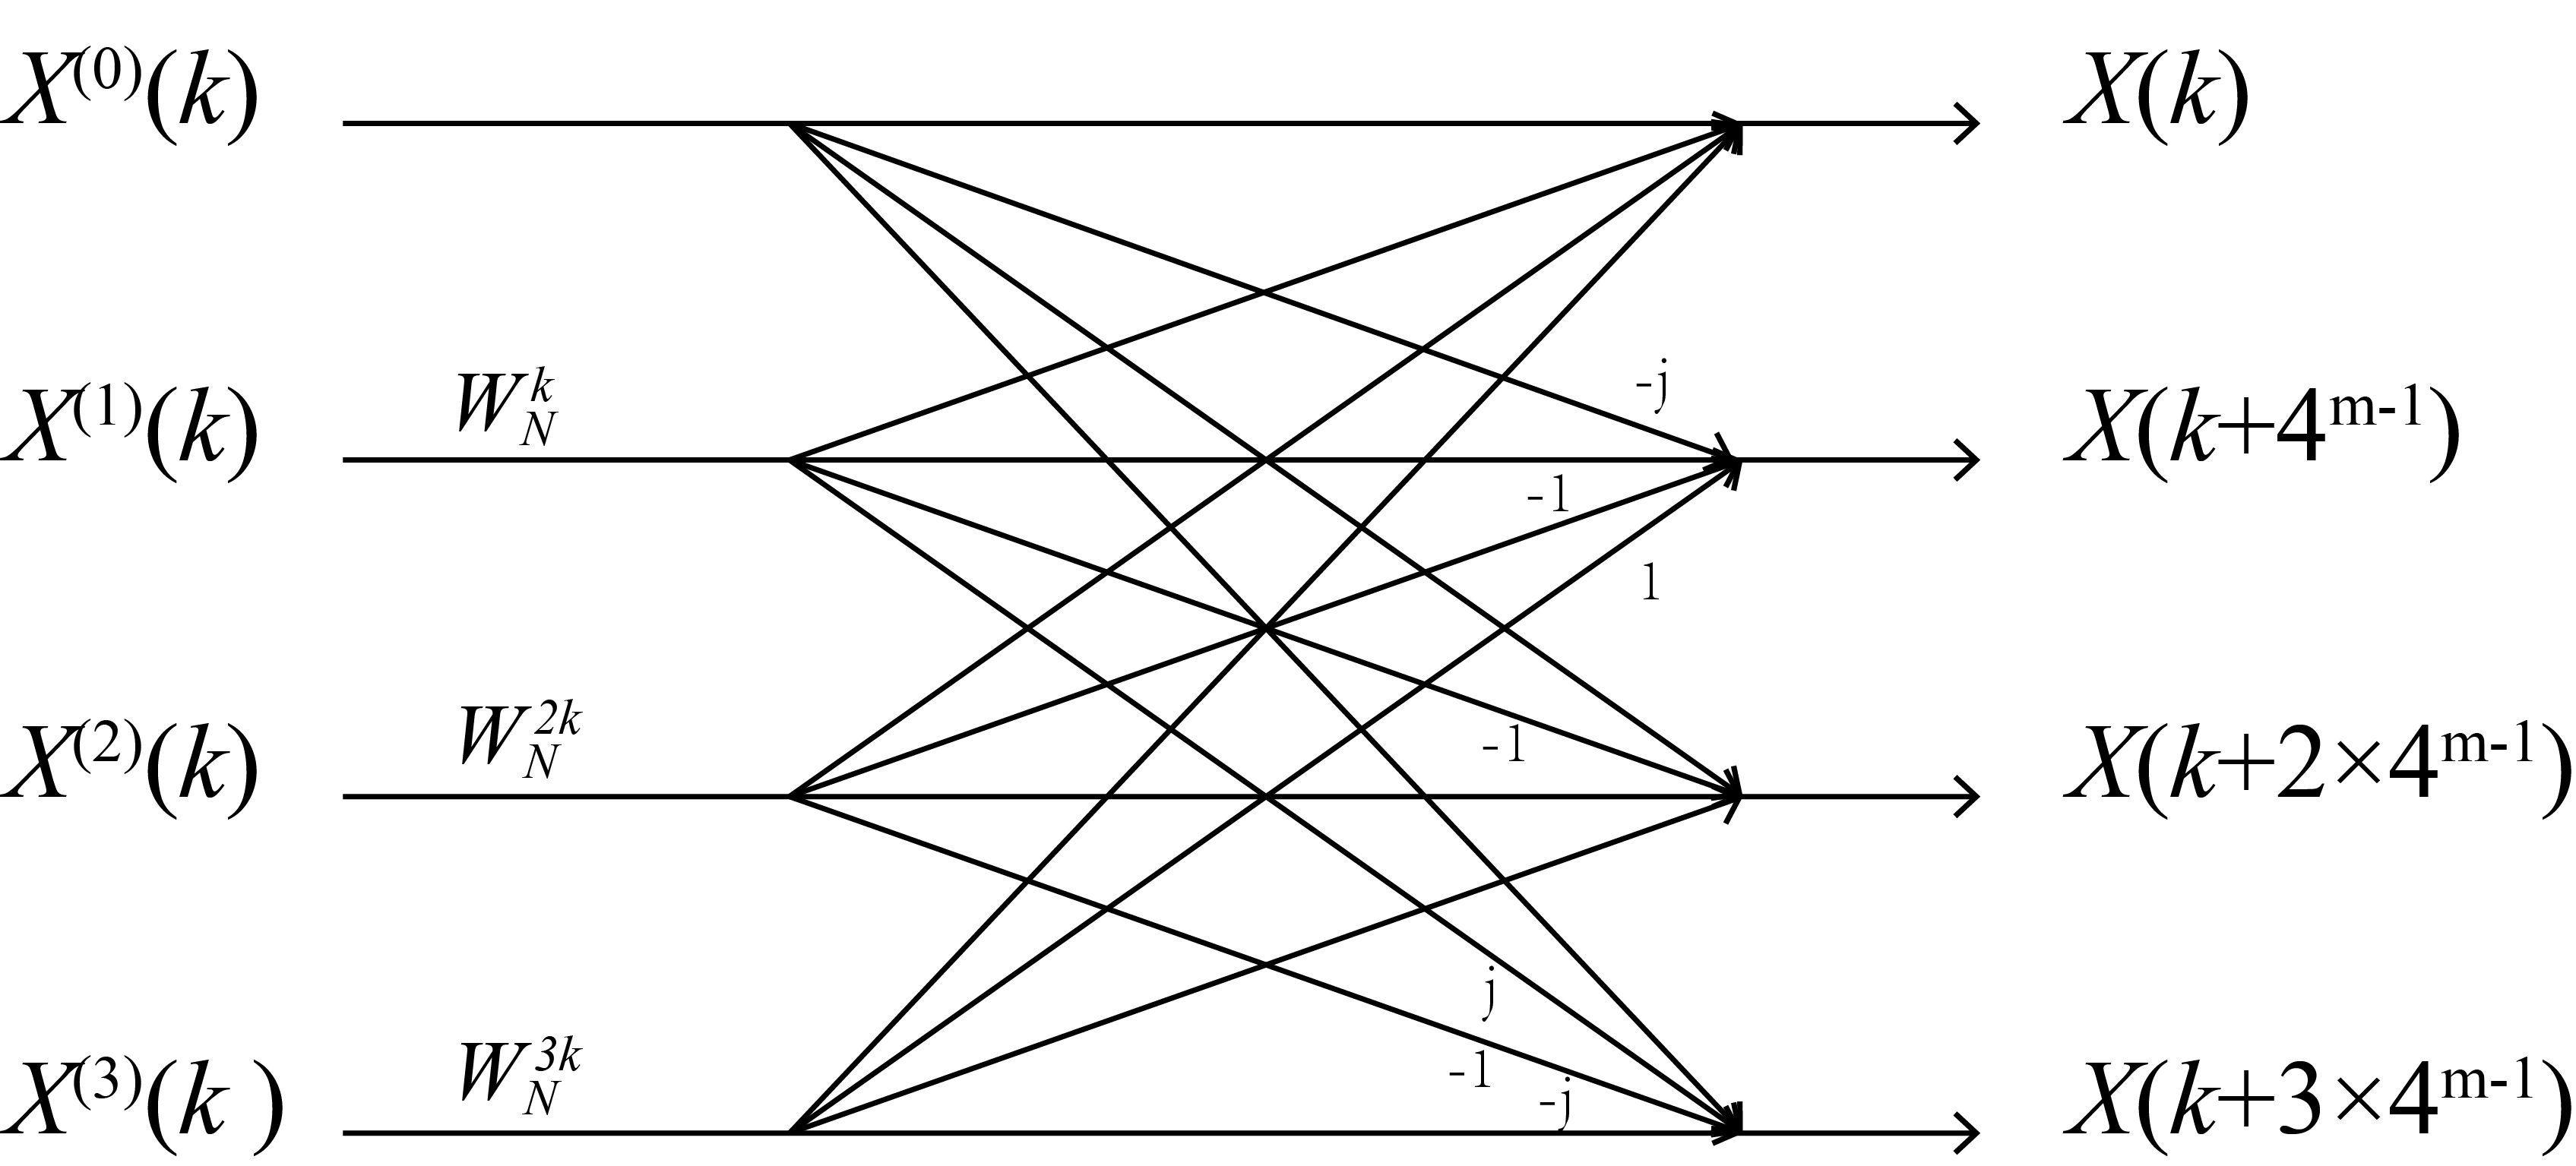
\includegraphics[width = 0.5\textwidth]{pic/butterfly1.png}
    \caption{基4  DIT-FFT中的蝶形运算}
\end{figure}
对于N点,基4DIT-FFT的整体计算过程如下:
\begin{figure}[H]
    \centering
    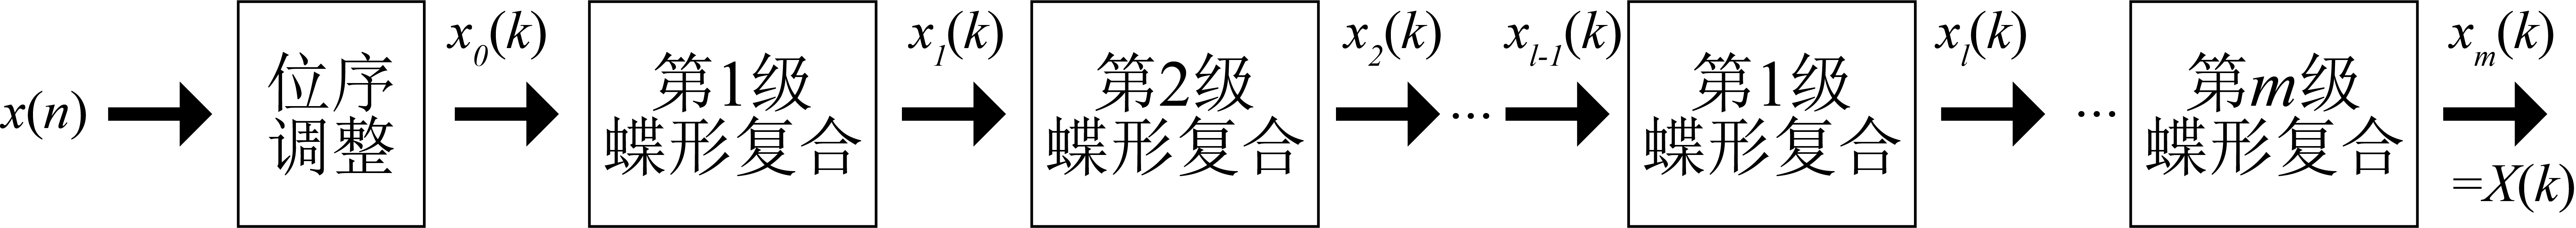
\includegraphics[width = 0.9\textwidth]{pic/butterfly2.png}
    \caption{基4  DIT-FFT计算过程}
\end{figure}
\subsection{16点基4-FFT算法的流图绘出如下(因绘图限制,省略系数-1,-j,j,具体系数对应项见上一蝶形图)}
\begin{figure}[H]
    \centering
    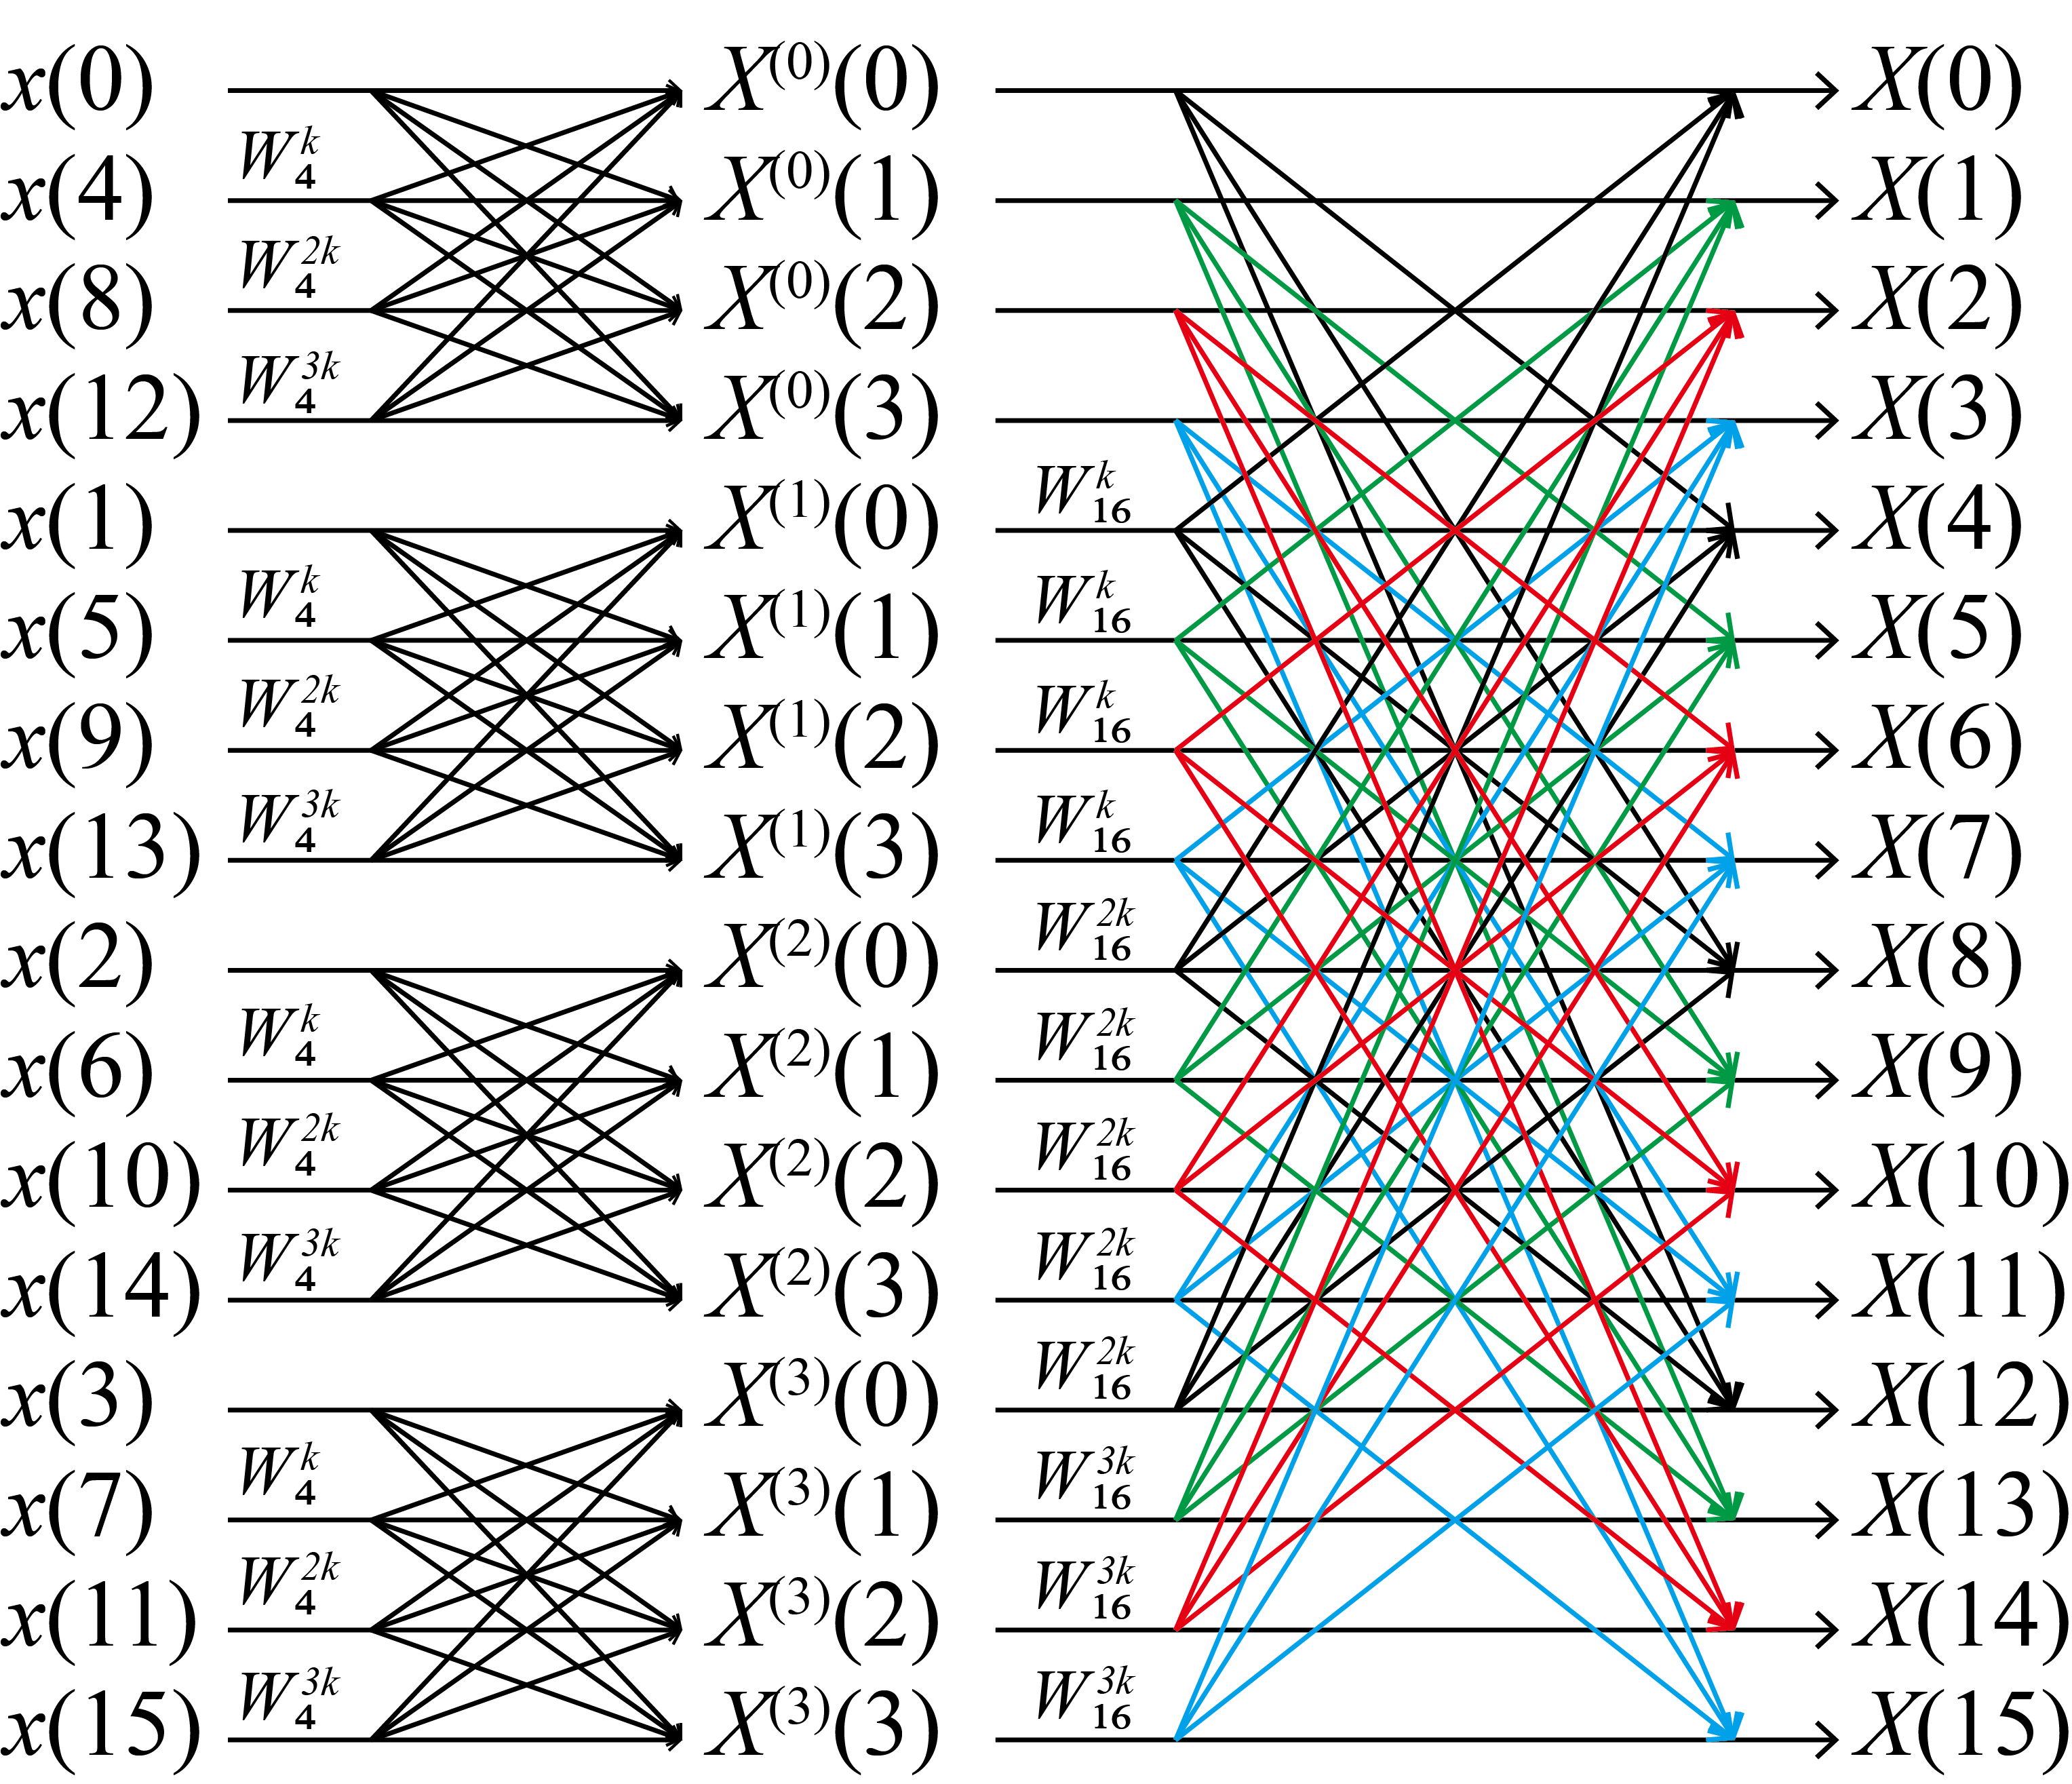
\includegraphics[width = 0.8\textwidth]{pic/butterfly3.png}
    \caption{16点基4-FFT算法的流图}
\end{figure}
\subsection{16点基4-FFT算法的MATLAB程序(studentname.m)列出如下}
\lstinputlisting[
    language       =   Matlab,
    title     =   {studentname.m}
]{src/studentname.m}
\subsection{用自己的学号构成的输入序列为(列出数值,插入图形)}
x(n) = [3, 1, 9, 0, 1, 0, 5, 5, 9, 7, 0, 0, 0, 0, 0, 0]
\begin{figure}[H]
    \centering
    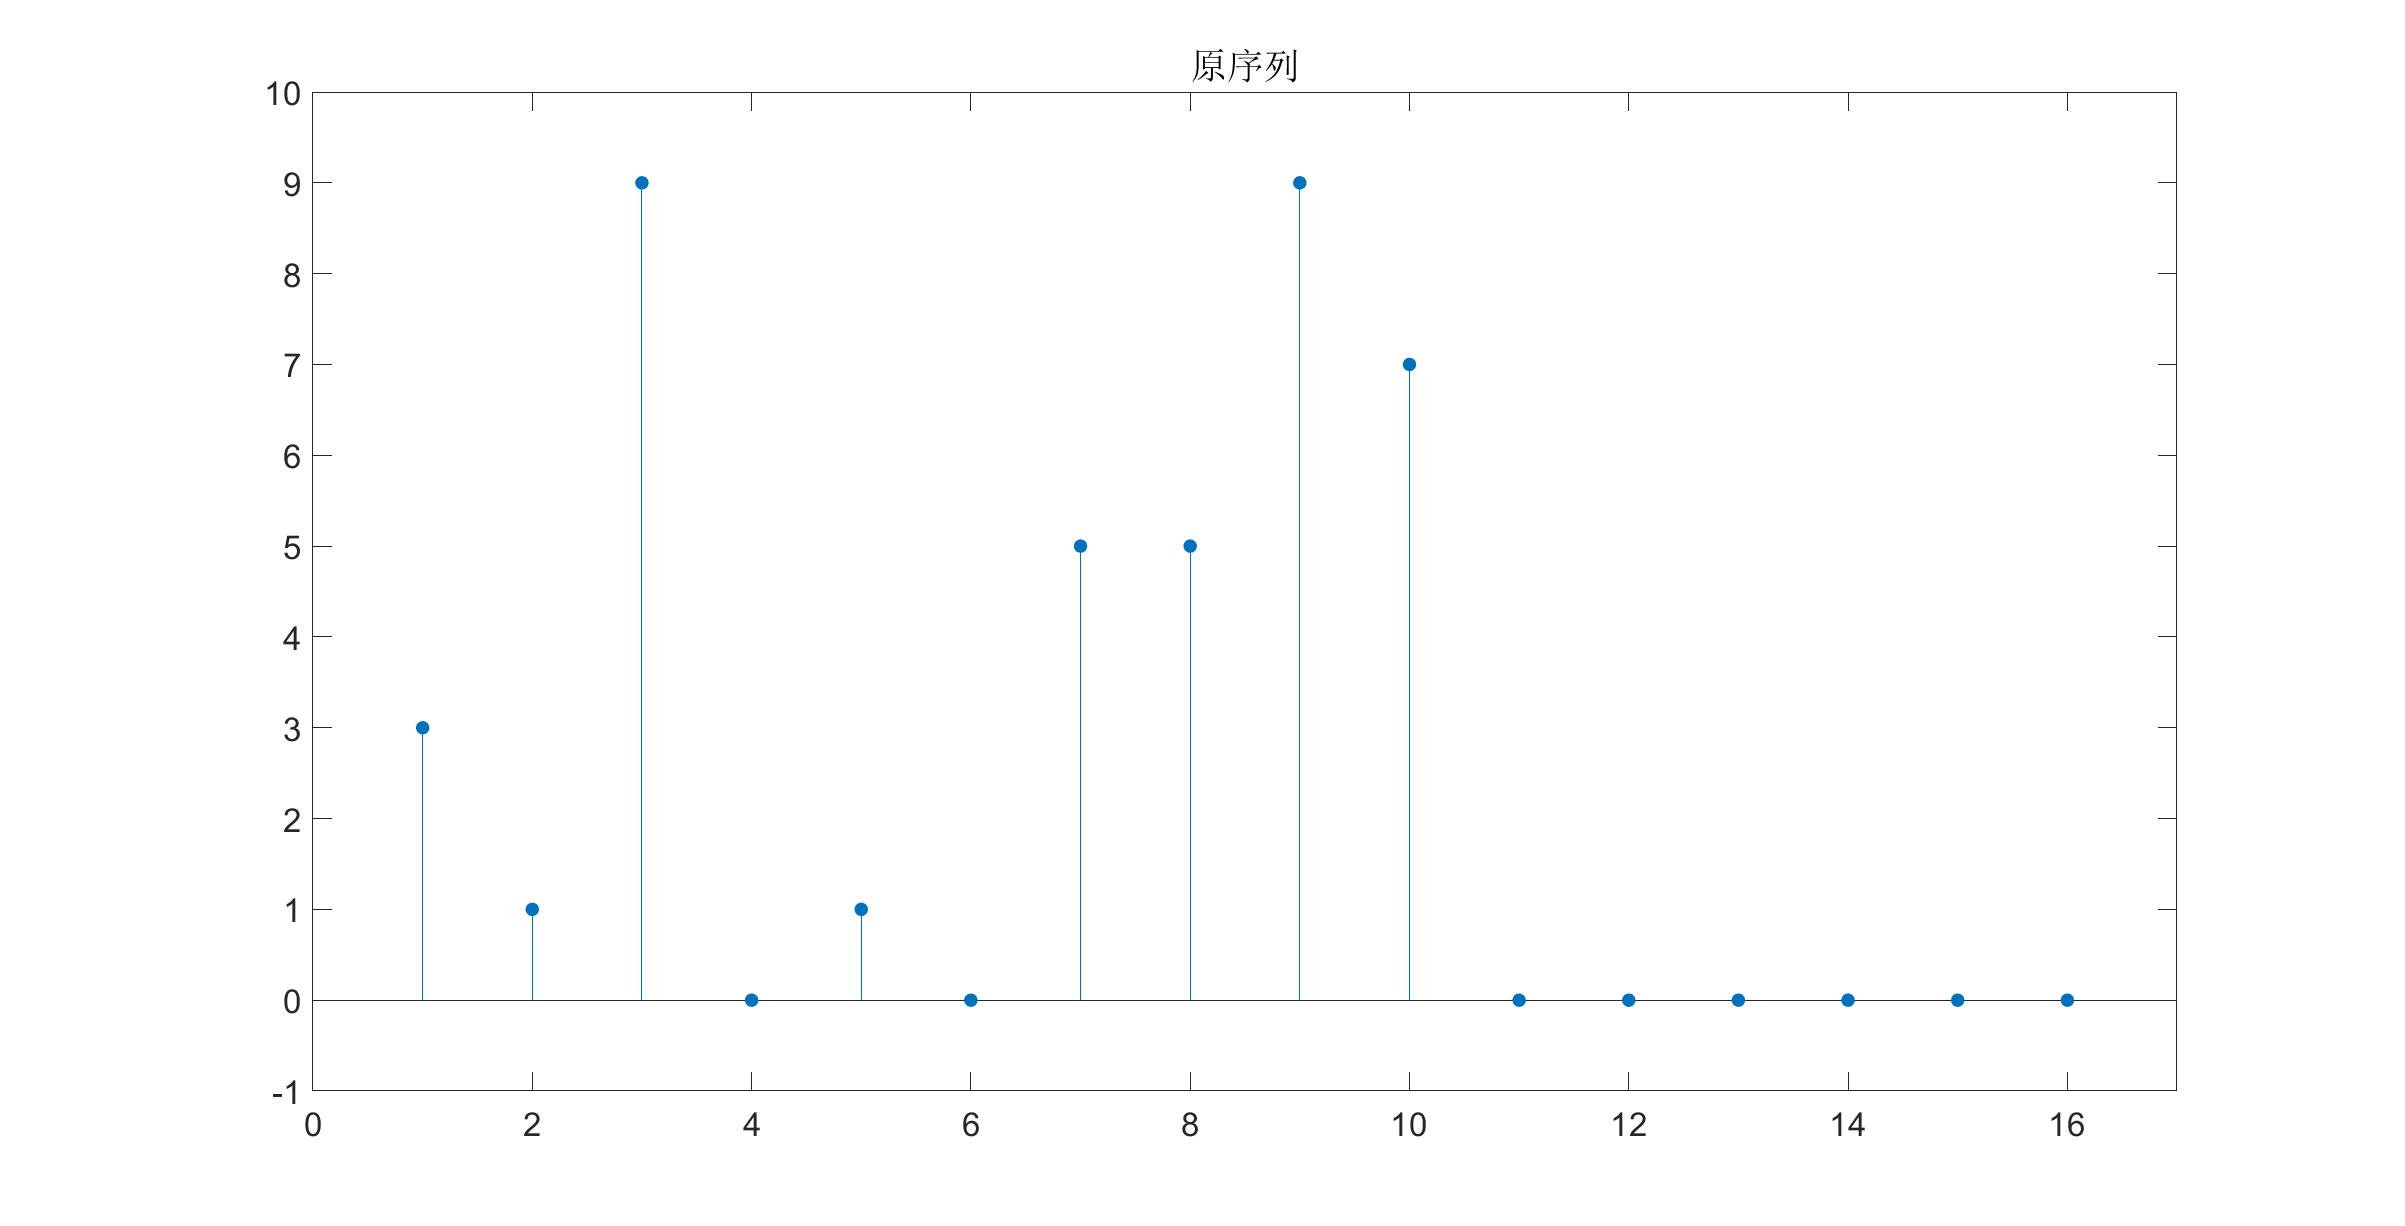
\includegraphics[width = 1.0\textwidth]{src/exp3_1.png}
\end{figure}
\subsection{对应的输出频谱序列为(列出数值,插入图形)}
Xk =

列 1 至 4

40.0000 + 0.0000i ,\, -13.3342 - 10.5168i ,\, 20.1924 - 6.1213i ,\, -13.0379 - 7.9756i

列 5 至 8

-1.0000 - 3.0000i ,\, -4.6189 + 9.8234i ,\, 1.8076 + 1.8787i ,\, 6.9911 + 11.2822i

列 9 至 12

14.0000 + 0.0000i ,\, 6.9911 -11.2822i ,\, 1.8076 - 1.8787i ,\, -4.6189 - 9.8234i

列 13 至 16

-1.0000 + 3.0000i ,\, -13.0379 + 7.9756i ,\, 0.1924 + 6.1213i ,\, -13.3342 + 10.5168i

\begin{figure}[H]
    \centering
    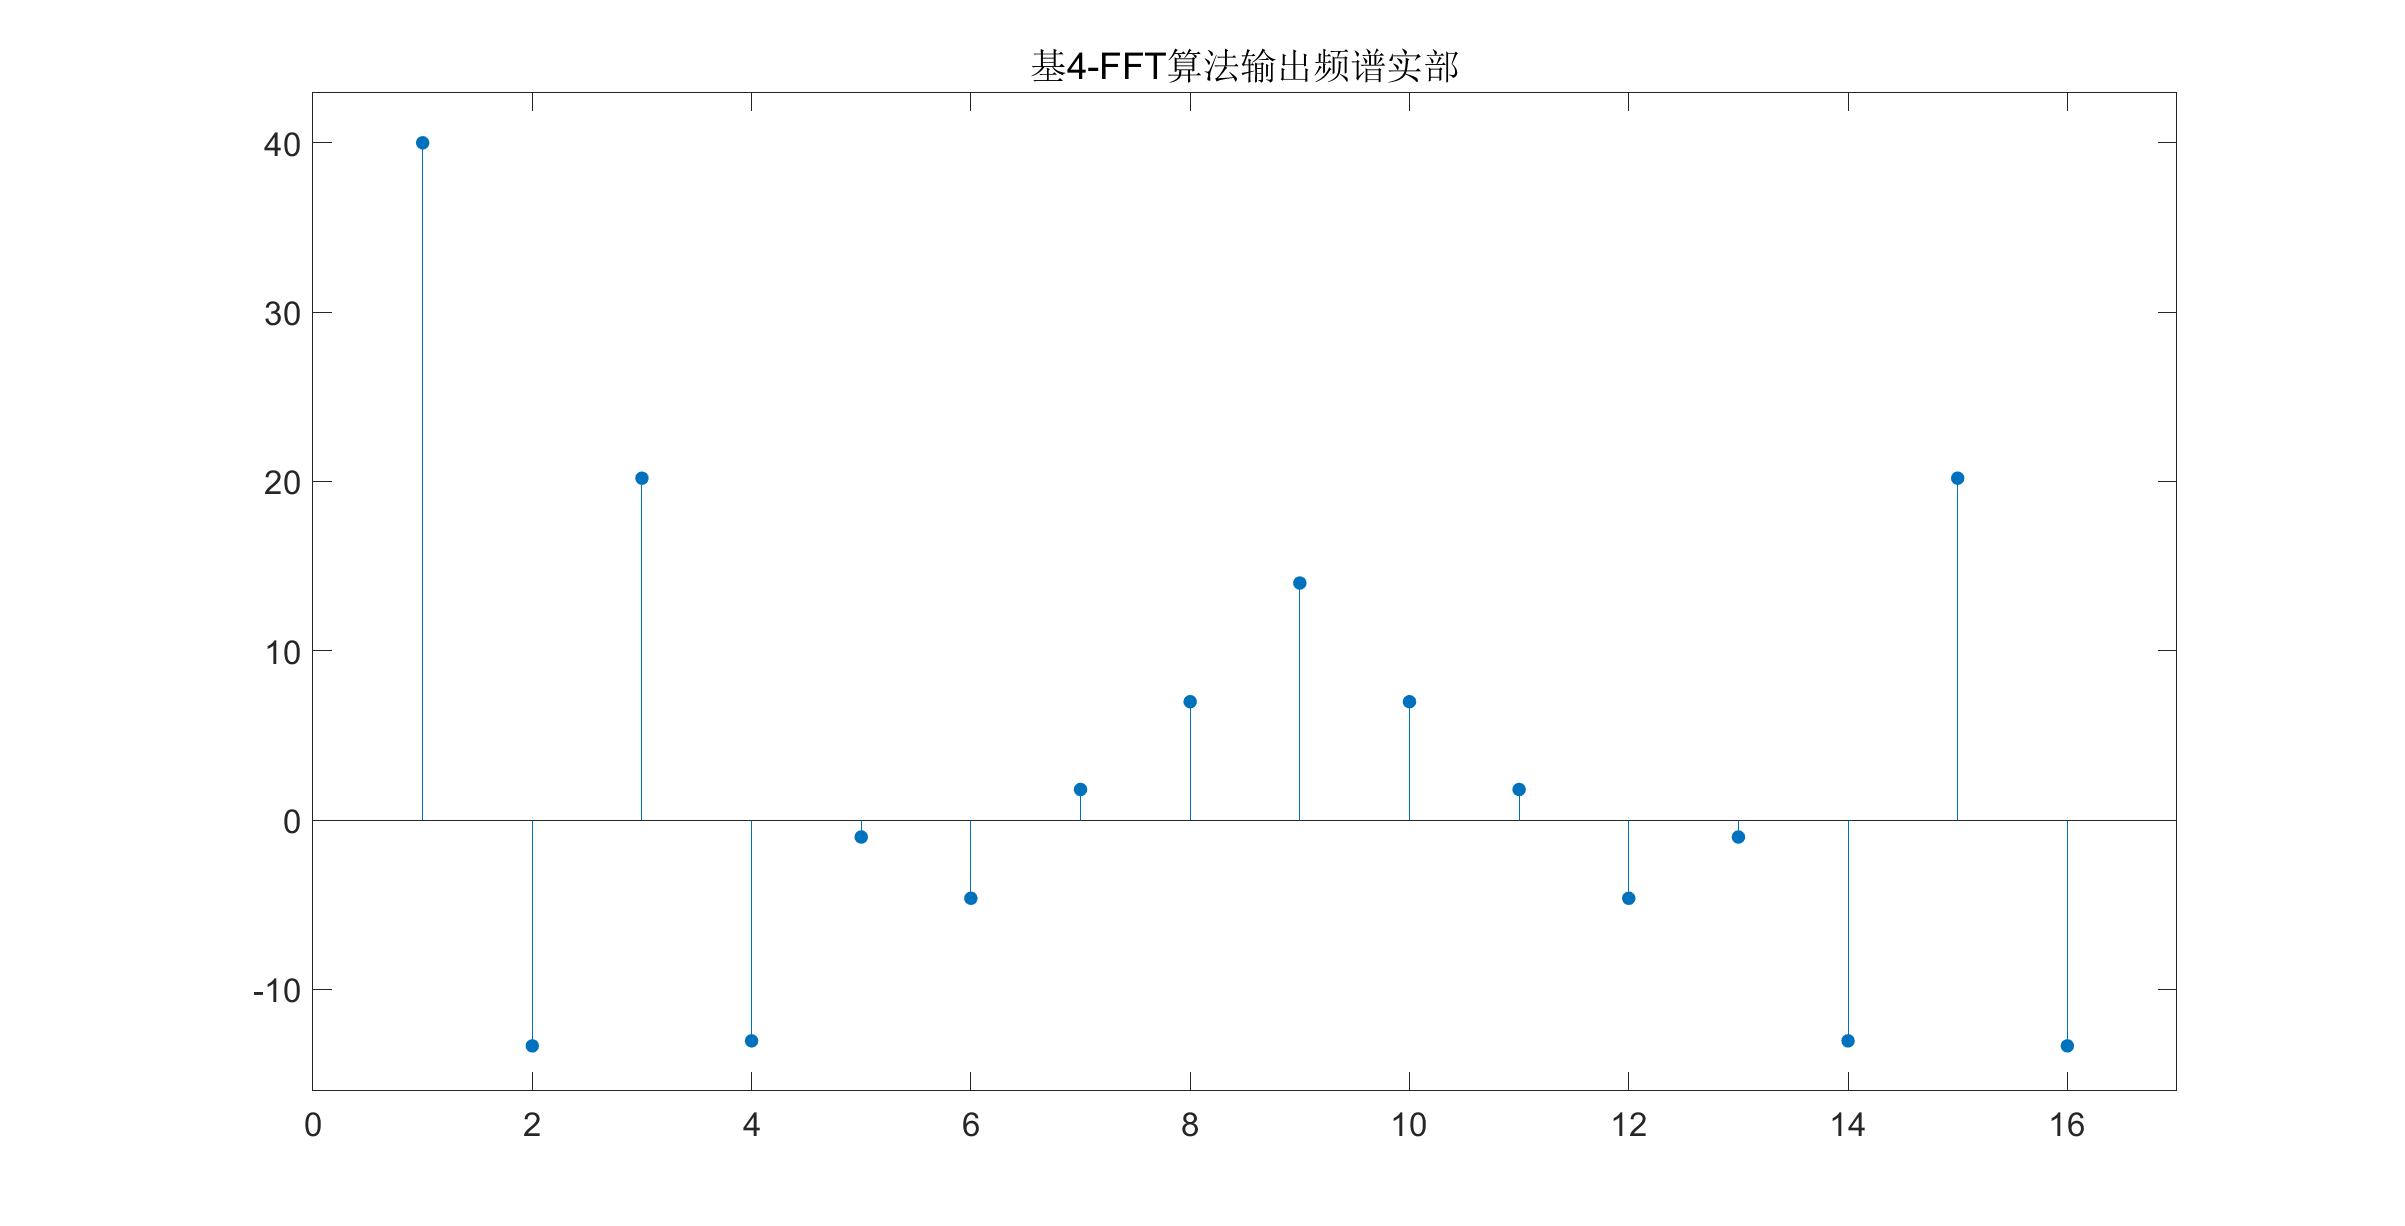
\includegraphics[width = 1.0\textwidth]{src/exp3_2.png}
    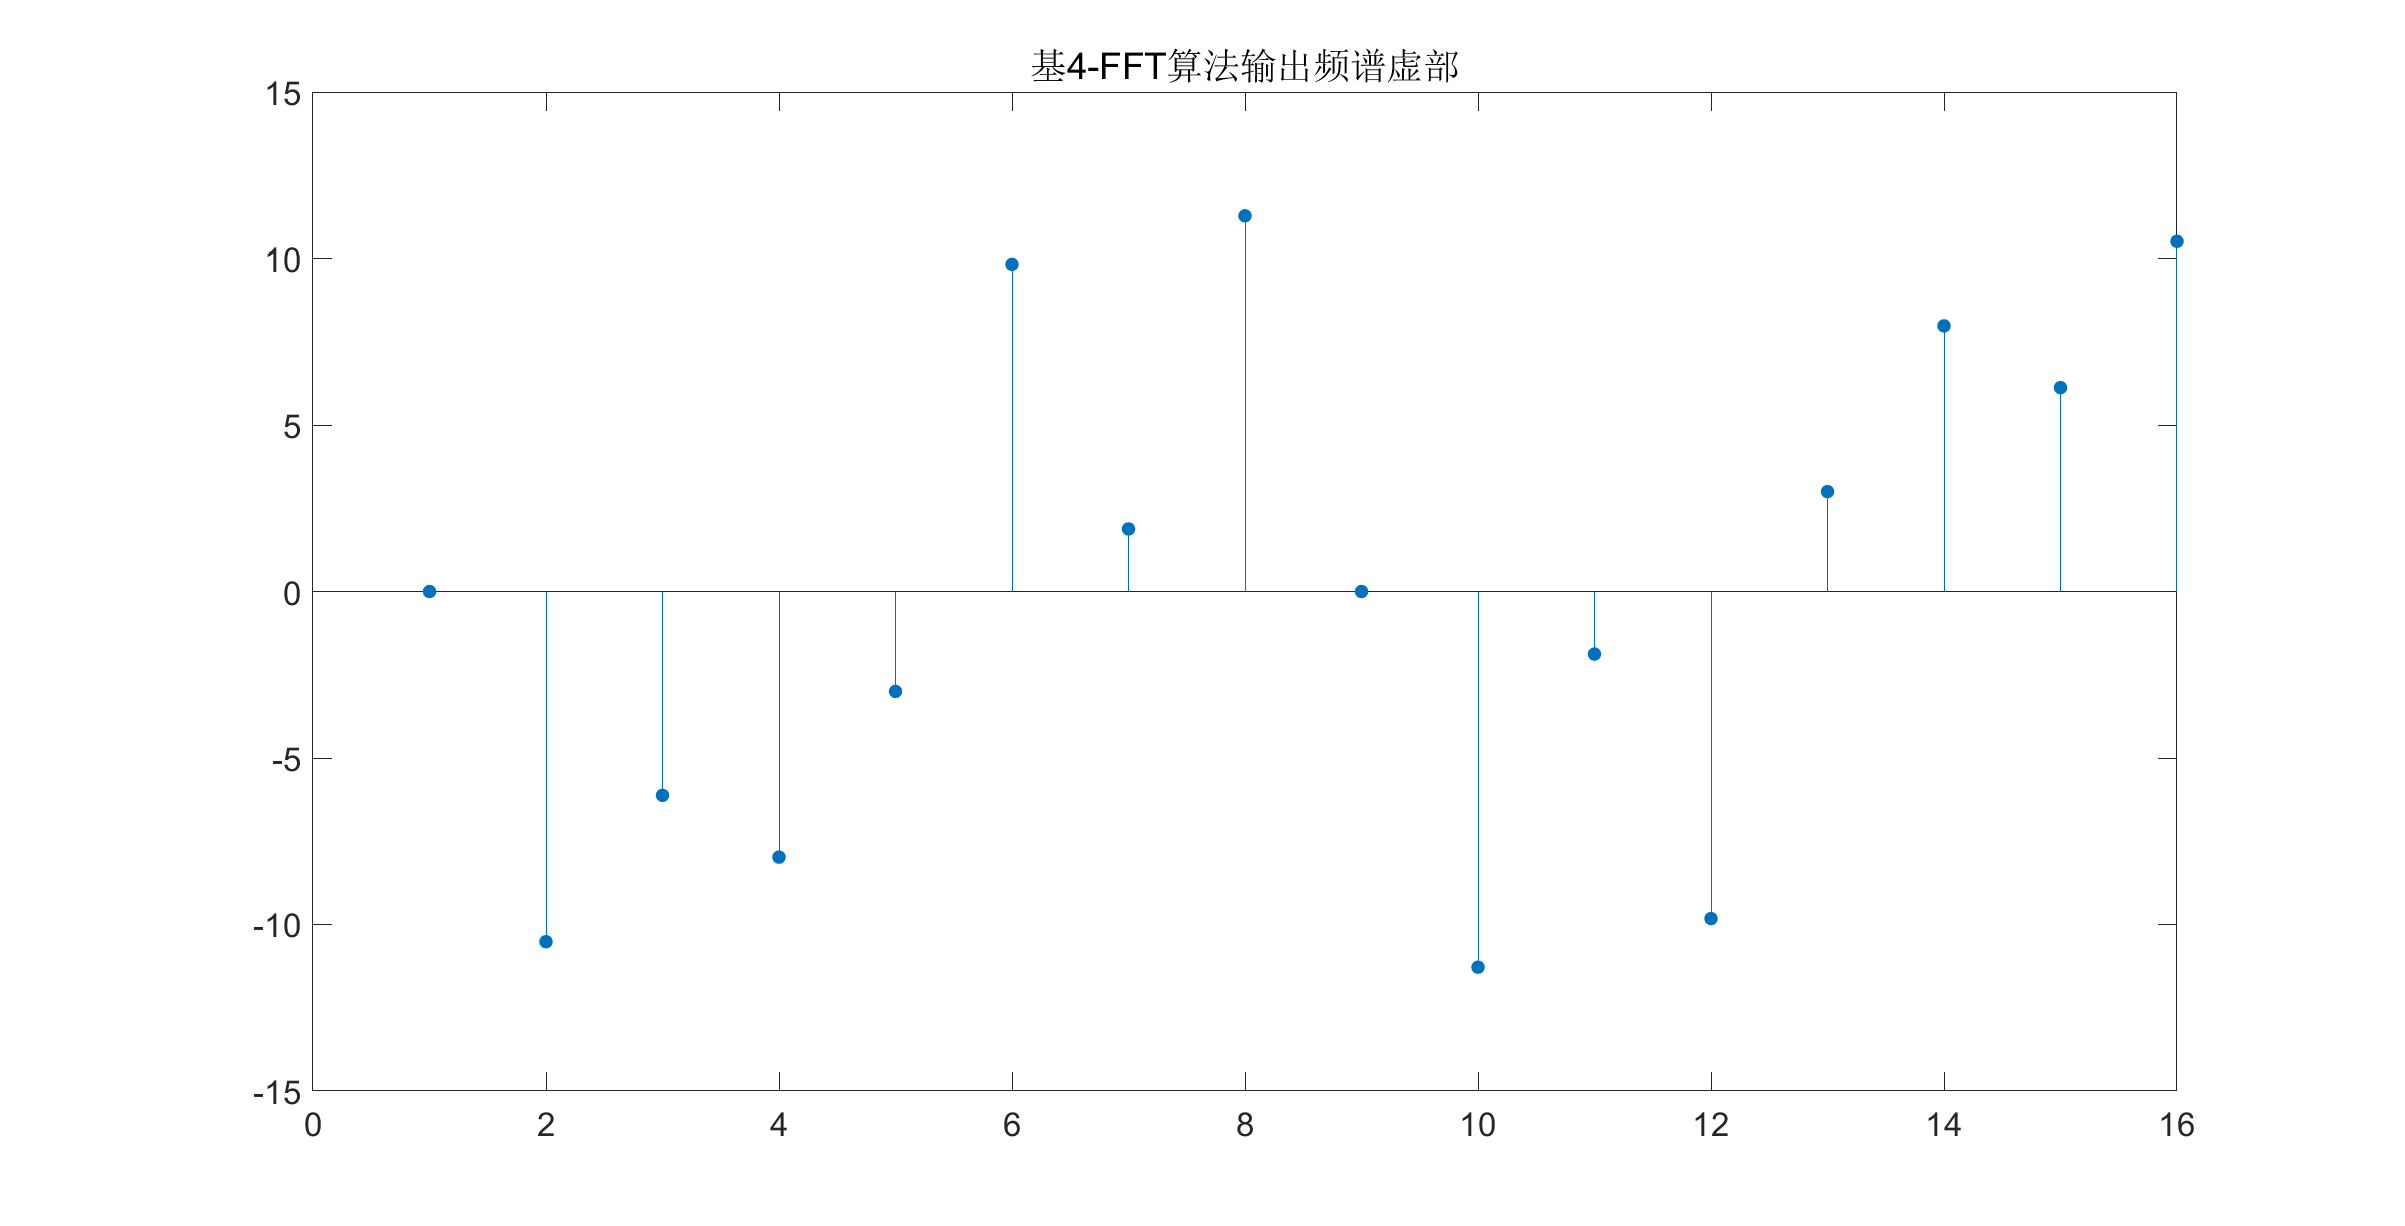
\includegraphics[width = 1.0\textwidth]{src/exp3_3.png}
\end{figure}
\section{实验结果与分析}
为了验证基4-FFT算法的正确性,我们直接调用了Matlab的fft函数进行了计算,其结果如下:
Xk2 =

列 1 至 4

40.0000 + 0.0000i ,\, -13.3342 - 10.5168i ,\, 20.1924 - 6.1213i ,\, -13.0379 - 7.9756i

列 5 至 8

-1.0000 - 3.0000i ,\, -4.6189 + 9.8234i ,\, 1.8076 + 1.8787i ,\, 6.9911 + 11.2822i

列 9 至 12

14.0000 + 0.0000i ,\, 6.9911 - 11.2822i ,\, 1.8076 - 1.8787i ,\, -4.6189 - 9.8234i

列 13 至 16

-1.0000 + 3.0000i ,\, -13.0379 + 7.9756i ,\, 20.1924 + 6.1213i ,\, -13.3342 + 10.5168i
\begin{figure}[H]
    \centering
    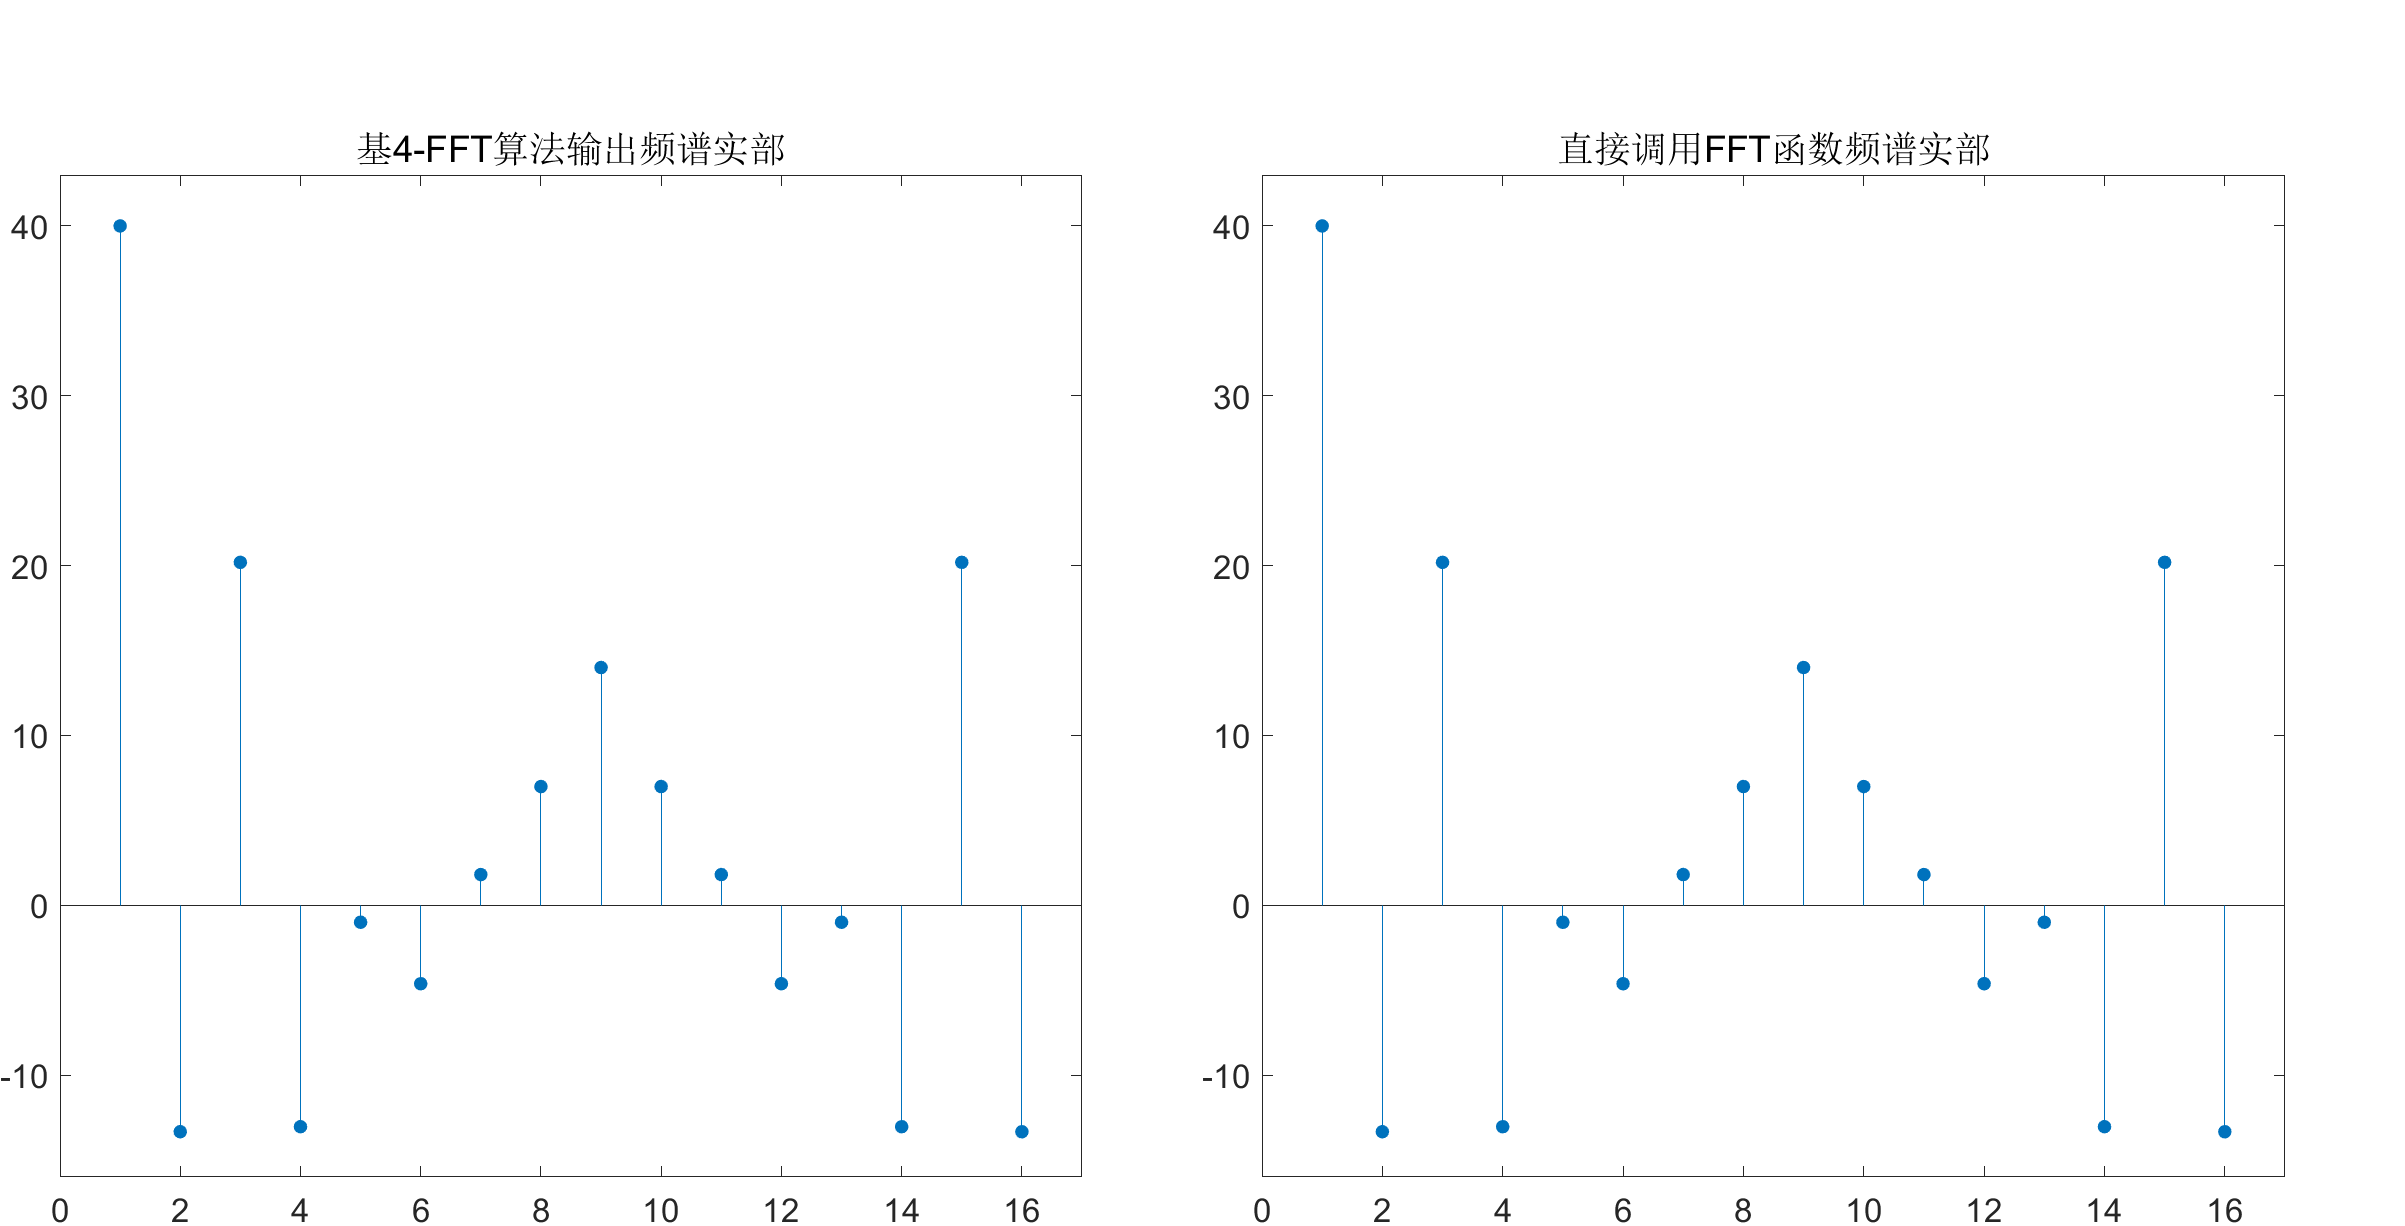
\includegraphics[width = 1.0\textwidth]{src/exp3_5.png}
    \caption{对比图}
\end{figure}
可看出Matlab的fft所得结果和自己的基于4-FFT算法所得结果一致,说明自己的结果的正确性。
\end{document}
